\documentclass[a4paper,12pt]{article}
\usepackage[utf8]{inputenc}
\usepackage[english]{babel}
\usepackage{authblk}
\usepackage{graphicx}
\usepackage{mathptmx}
\usepackage[singlespacing]{setspace}
\usepackage[headheight=1in,margin=1in]{geometry}
\usepackage{fancyhdr}
\usepackage[numbers]{natbib}
\usepackage{subcaption}

\renewcommand{\bibsection}{}
\renewcommand{\headrulewidth}{0pt}
\pagestyle{fancy}
\chead{%
  $6$$^{th}$ International Conference on Computational Social Science IC$^{2}$S$^{2}$\\
  July 17-20, 2020, 75 Amherst St. Cambridge, MA USA%
}

\graphicspath{{images/}}
\title{The Wisdom and Manipulability of Threads}
\author[]{} % Please leave Author-field blank for blind review and remove information that may identify the author(s)
\date{}

\begin{document}

\maketitle
\thispagestyle{fancy}

\vspace{-7em}
\begin{center}
\textbf{\textit{wisdom of crowds $|$ magnitude estimation $|$ decision-making $|$ threads $|$  dot-guessing games}}
\newline
\end{center}
%\vspace{-2em}

\section*{Extended Abstract}
Social decision-making is increasingly relying on digitized aggregates of people’s opinions and judgments. These aggregates are frequently maintained as threads, i.e. as sequences of posts on a website. While it has been shown that knowledge of thread aggregates can distort individual decision-making, it is unknown how the ability to see preceding posts in a thread may influence collective accuracy, i.e. the wisdom of threads. We investigate experimentally the accuracy and manipulability of threads, in which people make numerical estimates of varying difficulty and varying degrees of social information. Analyzing the data using gaussian mixture models (GMMs), we obtain novel insights into the intrinsic use of social information within
each thread.

The data was collected from 7,814 participants playing a dot-guessing game \cite{horton2010dot} on Amazon Mechanical Turk, where each participant successively estimated the number of visible dots $d \in \{55,148,403,1097\}$ in various images, while seeing $v \in \{0,1,3,9\}$ preceding estimates (historical threads). An additional 3,934 participants were shown the same images while seeing the $v \in \{1,3,9\}$ \textit{highest} estimates made so far (manipulated threads). 

We compare the log-ratio of the individual thread medians, $\log(M_{(d,v)}/d)$, using a linear normal model to quantify differences between threads in terms of $\log(d)$ and $v$, the latter as a categorical variable. Figure \ref{fig: median confidence bounds - historic} shows that the collective performance for historical threads declines significantly with increasing task difficulty (higher $d$), but improves when the social information is substantial (high $v$). In contrast to \cite{lorenz2011social} and in accordance with \cite{becker2017network}, this finding supports the claim that crowds indeed may become wise under (pristine) social influence. For the manipulated series, Fig.\ref{fig: median confidence bounds - manipulated}, the manipulation gives a large positive bias for $v=3,9$ which increases with $d$, implying that when a task becomes more demanding, the amount of (biased) social information has a detrimental impact on thread performance.

\begin{figure*}[!b]
\centering
	\begin{subfigure}[t]{.46\linewidth}
		\centering
		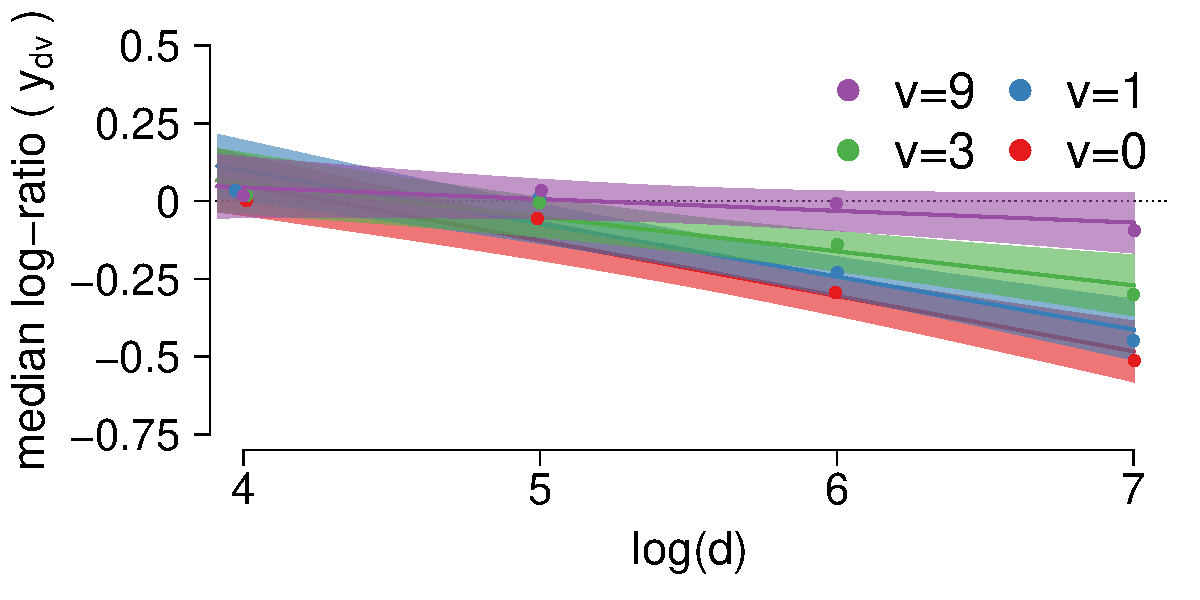
\includegraphics[width=1\linewidth]{med_confidence_h.pdf}	
		\caption{\footnotesize Historical threads.}
		\label{fig: median confidence bounds - historic}
	\end{subfigure}
	\begin{subfigure}[t]{.46\linewidth}
		\centering
		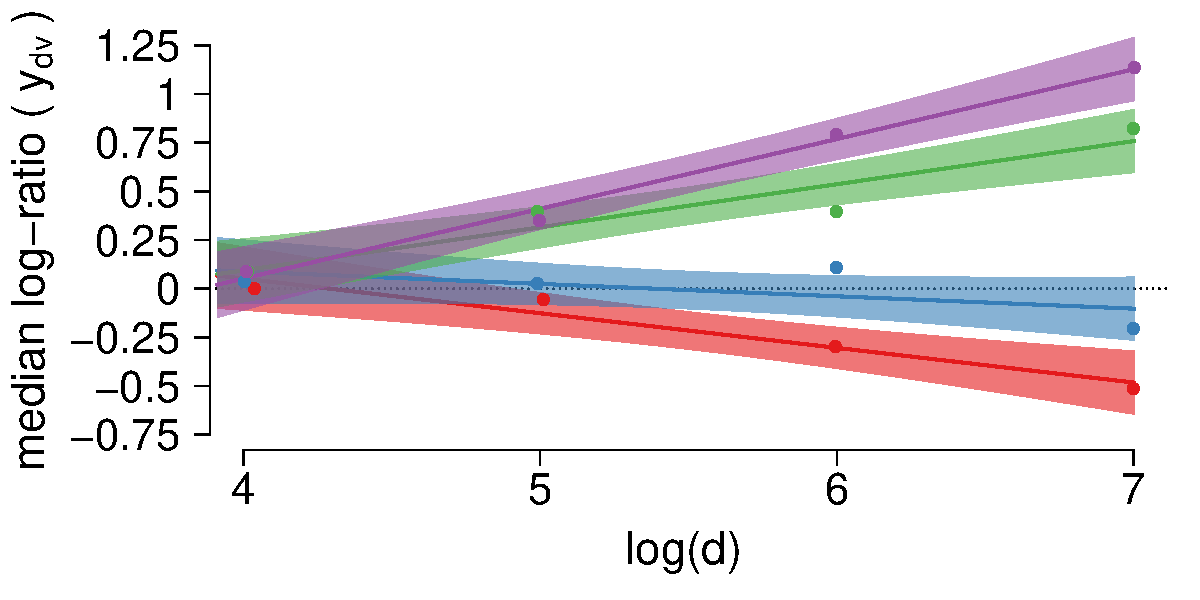
\includegraphics[width=1\linewidth]{med_confidence_m.pdf}		
		\caption{\footnotesize Manipulated threads.}
		\label{fig: median confidence bounds - manipulated}
	\end{subfigure}
	\caption{\footnotesize Relationship between median log-ratio and number of dots (lines) with 95\% confidence bounds (shaded areas). The colors represent the four settings on number of visible estimates. There is a clear relation between number of dots and number of visible estimates in both thread types, but it is more pronounced for the manipulated series. The red lines corresponding to the control groups with $v=0$ are the same in both plots.}
	\label{fig: median confidence bounds}
\end{figure*}

\begin{figure*}[!ht]
	\centering
	\begin{subfigure}[t]{.44\linewidth}
		\centering
		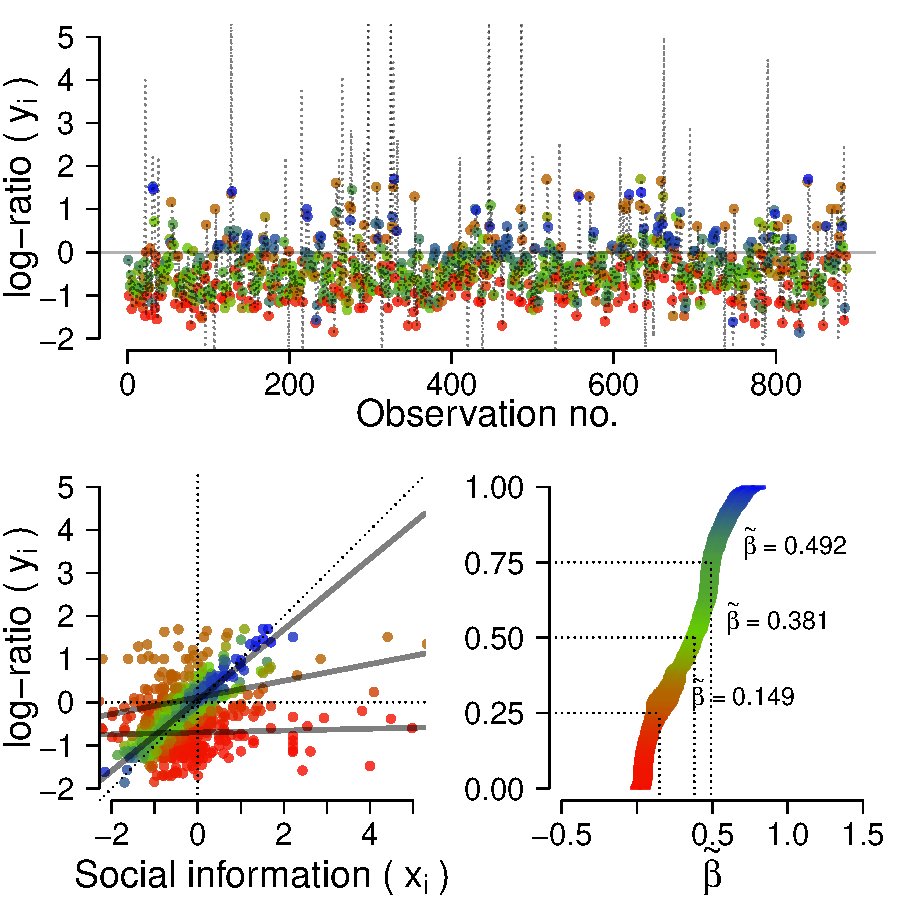
\includegraphics[width=1\linewidth]{h10971.pdf}
		\caption{\footnotesize Historical thread with $d=1097$ and $v=1$}
		\label{fig: h d=1097, v=1}
	\end{subfigure}
	\begin{subfigure}[t]{.44\linewidth}
		\centering
		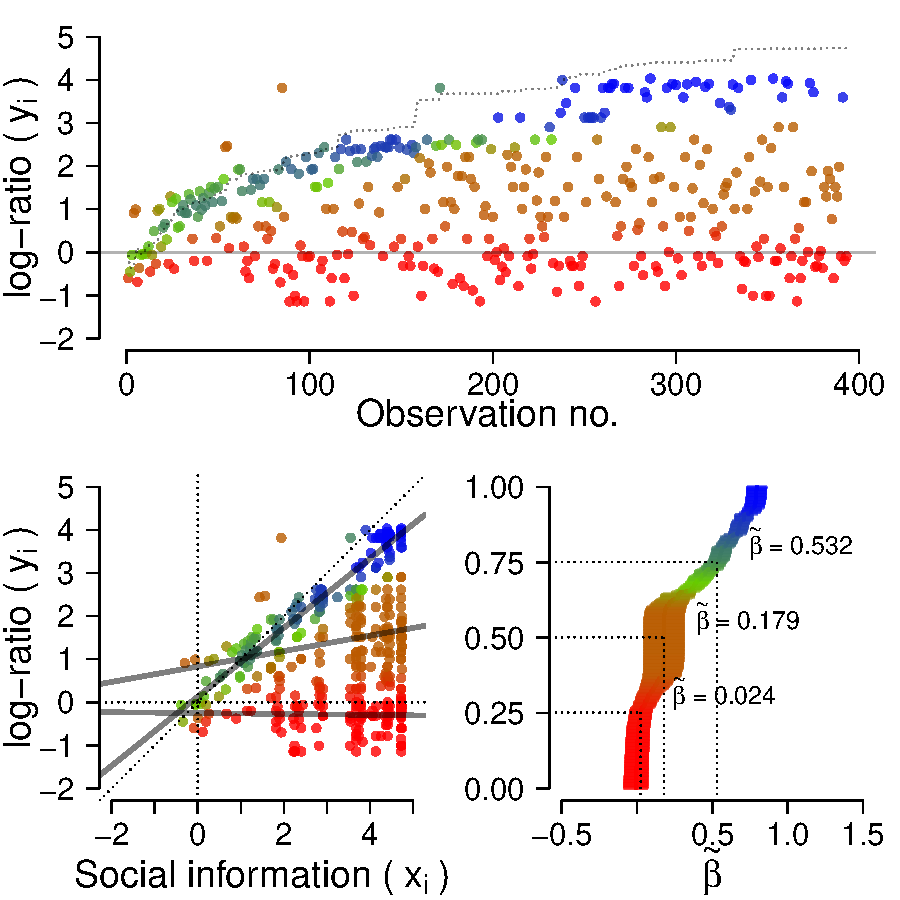
\includegraphics[width=1\linewidth]{m10979.pdf}
		\caption{\footnotesize Manipulated thread with $d=1097$ and $v=9$}
		\label{fig: m d=1097, v=9}
	\end{subfigure}
	\begin{subfigure}[t]{.1\linewidth}
		\centering
		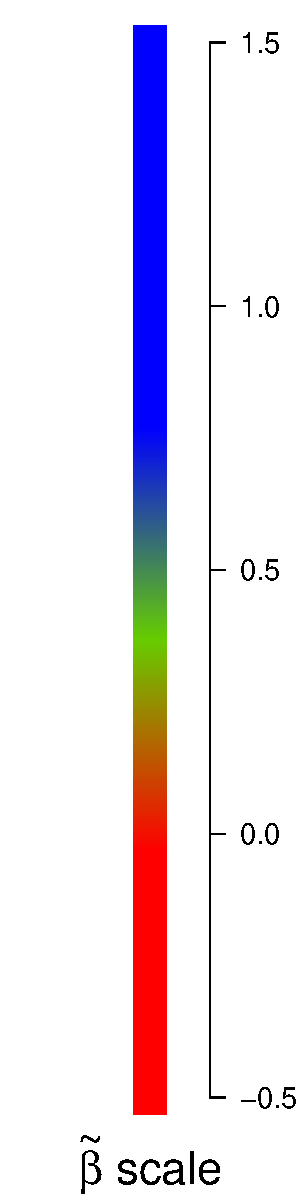
\includegraphics[width=1\linewidth]{betascale.pdf}
	\end{subfigure}
	\caption{\footnotesize The left hand side shows three plots of a historical thread with $d=1097$ and $v=1$, and the right hand side shows three plots of a manipulated thread with $d=1097$ and $v=9$. Top plots shows the log-ratio estimates over time (observation no.), with the geometric mean of the social information shown by a dotted line. Bottom left plots show the log-ratio of the estimates as a function of the log-ratio of the social information, indicating how differently participants use their social information. Bottom right plots show the cumulative distribution of individual $\tilde{\beta}$'s with 95\% intervals derived from the fitted models and added interquartile values of $\tilde{\beta}$.}
	\label{fig: social influence}
\end{figure*}
Figure \ref{fig: social influence} displays the effect of social information, obtained by fitting a GMM to each thread using the geometric mean of visible estimates as a proxy for the available social information. The effect of social information on each participant is given by $\tilde{\beta}$, the weighted average of the individual states of the GMM, where a high value ($\tilde{\beta}>0.6$, blue color) implies a large effect, a low value ($\tilde{\beta}\approx 0$, red color) implies little or no effect and a medium value ($\tilde{\beta} \approx 0.4$, green color) suggests a compromise between the two extremes. Figure \ref{fig: h d=1097, v=1} shows results for a historical thread where estimates are split among keepers (red), compromisers (green) and adopters (blue) throughout the thread. Figure \ref{fig: m d=1097, v=9} in contrast shows the results for a manipulated thread, where the same three groups are clearly visible, but the evolutionary trend is completely different compared to the historical thread. Contrasting Figures \ref{fig: h d=1097, v=1} and \ref{fig: m d=1097, v=9} clearly reveals different dynamics of threads in terms of manipulation or not. In general, our experiments show distinct distributions of overlapping groups (keepers, compromisers and adopters) in each thread, and in the case of manipulation suggest a substantial split into enthusiastic adopters versus skeptic keepers. The GMM framework is also applied to independent data from \cite{jayles2017social} allowing similar insights into qualitatively different tasks. 

%\vspace{-1em}
\setlength{\bibsep}{0.0pt}
\bibliographystyle{model1-num-names}
\bibliography{wamot}

\end{document}
